\documentclass[ignorenonframetext,10pt,aspectratio=169]{beamer}

\usepackage{umut}
\usepackage{umuttr}
\usepackage{usynsem}
\usepackage[utf8]{inputenc}
\usepackage{uling}
\usepackage{natbib,unatbib}
\usepackage{linguex}
         \renewcommand{\refdash}{}
\usepackage{ubeamer}
\usepackage{verbatim}

\usepackage{fancyvrb}

\usepackage{tikz-qtree}
\usetikzlibrary{er,positioning}

\title{Constituent structure}
\author{\ \\ \vspace{20pt} Umut \"Ozge\\  }

\date{COGS 532: Theoretical Linguistics\\ METU, Informatics}

\begin{document}

\begin{frame}\frametitle{}
\thispagestyle{empty}
\maketitle
\end{frame}

\begin{frame}[t,plain]{}

\end{frame}

\begin{frame}[t,plain]{}

\end{frame}

\begin{frame}[t,plain]{}

\ex. John saw the man with the telescope.


\end{frame}

\begin{frame}[t,plain]{}

\ex. John saw the man with the telescope.

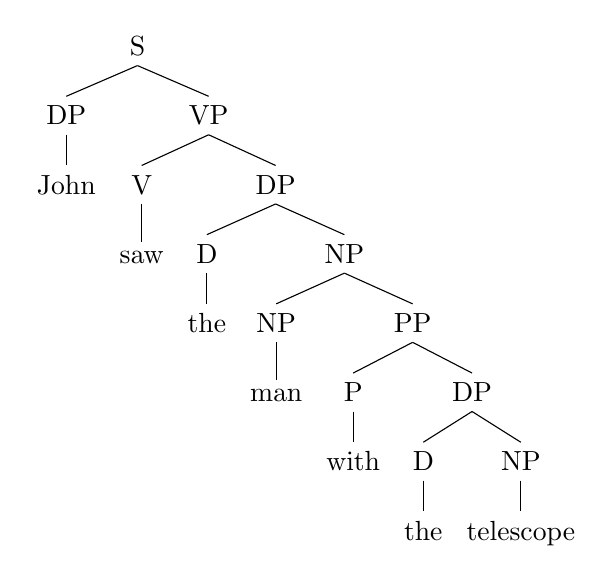
\begin{tikzpicture}
	\tikzset{level distance=25pt}
	\Tree [.\sysm{S}
		[.\sysm{DP} John ]
		[.\sysm{VP}
			[.\sysm{V} saw ]
			[.\sysm{DP}
				[.\sysm{D} the ]
				[.\sysm{NP} 
					[.\sysm{NP} man ]
					[.\sysm{PP}
						[.\sysm{P} with ]
						[.\sysm{DP} 
							[.\sysm{D} the ]
							[.\sysm{NP} telescope ]
						]
					]	
				]
			]
		]
	]
\end{tikzpicture}
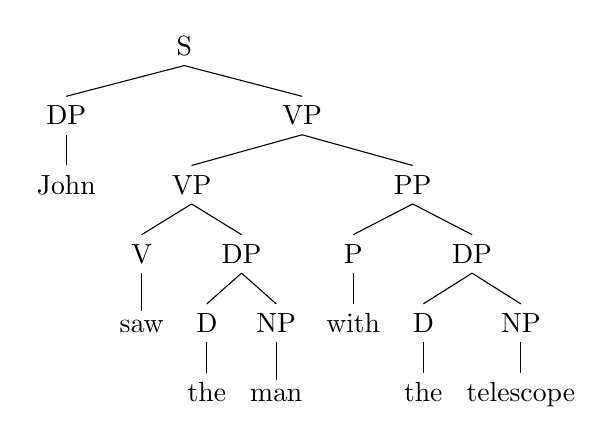
\begin{tikzpicture}
\tikzset{level distance=25pt}
	\Tree [.\sysm{S}
		[.\sysm{DP} John ]
		[.\sysm{VP}
			[.\sysm{VP}
				[.\sysm{V} saw ]
				[.\sysm{DP}
					[.\sysm{D} the ]
					[.\sysm{NP} man ]
				]
			]
			[.\sysm{PP}
				[.\sysm{P} with ]
				[.\sysm{DP} 
					[.\sysm{D} the ]
					[.\sysm{NP} telescope ]
				]
			]	
		]
	]
\end{tikzpicture}
\end{frame}

\begin{frame}[t,plain]{}

\end{frame}

\begin{frame}[t,plain]{}

\end{frame}

\end{document}
